\documentclass{article}

\usepackage[utf8]{inputenc}
\usepackage[danish]{babel}
\usepackage{float}
\usepackage{fancyhdr}
\usepackage{amsmath}
\usepackage{color}
\usepackage{listings}
\usepackage{graphicx}
\usepackage{pdfpages}
\usepackage{booktabs}
%\usepackage{enumitem}
\usepackage[a4paper, top = 1in, bottom = 1in, left=1in,right=1in]{geometry}

\title{Tællende Aktivitet 2}
\author{Peter Heilbo Ratgen \\ perat17}
\date{\today}

\begin{document}
\maketitle

\section{Opgave 1}
\subsection{Deskriptiv analyse}
En deskriptiv analyse af udgifterne til behandling af patienter 
\textsc{Treatcost}. 
\begin{figure}[h]
  \centering
  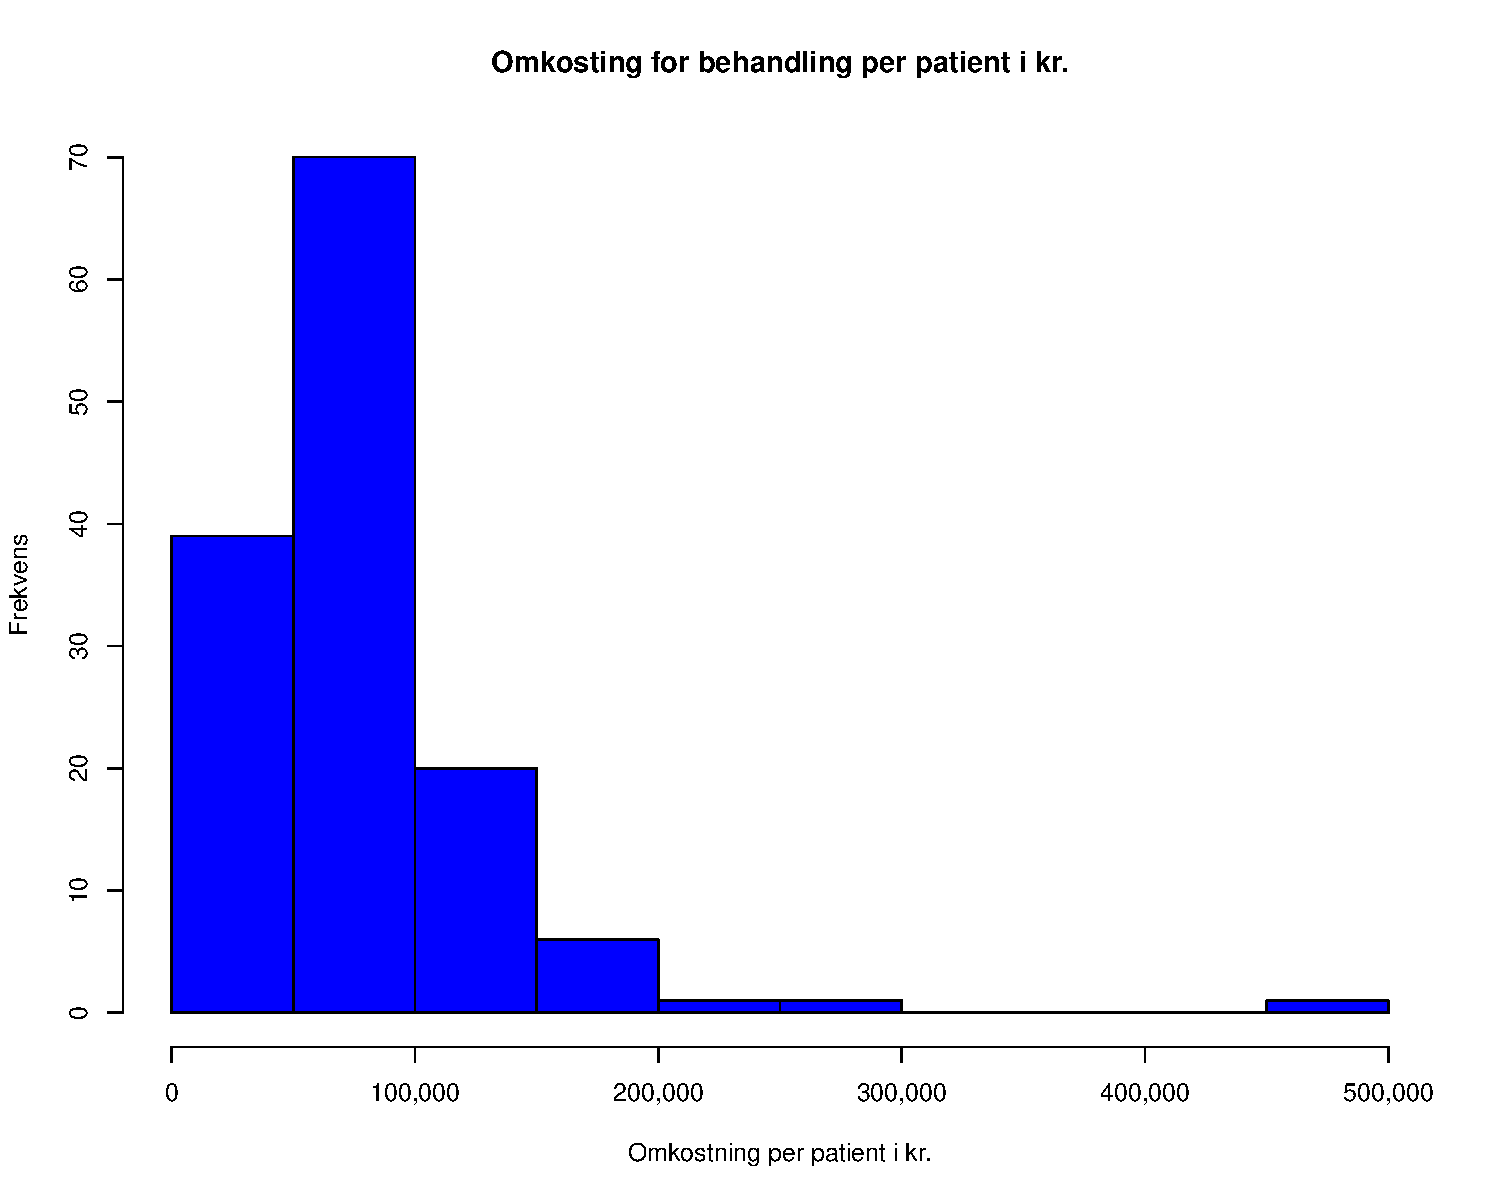
\includegraphics[width=0.6\textwidth]{./plots/treatcost.pdf}
  \caption{Histogram af omkostningen for at behandle patienter}
\end{figure}



% Histogram
% Summering af nøgletal
% Modus
% Standardafvigelse


% Konklusion


\section*{Opgave 2}

% Konklusion

\section*{Opgave 3}

Vi skal elimiere de varibler der ikke er ikke er vigtige for modellen, da den
mest komplekse model (den fulde model) ikke altid er den bedste. Til at
eliminere variabler og maksimere $ R^2_{adj} $ elimineres de variabler der ved
eliminering giver den højeste $ R^2_{adj} $. 
% Konklusion

\section*{Opgave 4}

Vi har en hypotese om at regionale forskellige kan have en indflydelse på brugen
af respirator, og de udgifter der følger med.

$ H_0 $: Der er ingen regionale forskelle i brugen af respirator.
$ H_1 $: Der er regionale forskelle i brugen af respirator.

% Konklusion

\section*{Opgave 5}

Vi har en hypotese om at bestemte udgifter kan være relateret til køn, vi skal
undersøge om middeludgifterne til røntgenundersøgelser er højere for mandlige
end kvindelig patienter.


% Konklusion

\end{document}

